\documentclass[a4paper, 11pt]{article}

\usepackage[utf8]{inputenc}

\usepackage[T1]{fontenc}

\usepackage[english]{babel}

\usepackage{graphicx}

\usepackage{multicol}

\usepackage{floatrow}

\usepackage[margin = 1in]{geometry}

\usepackage{float}

\usepackage[hidelinks, urlcolor=cyan]{hyperref}

\usepackage{url}

\usepackage{natbib}

\bibliographystyle{abbrvnat}
\setcitestyle{authoryear,open={(},close={)}}

\usepackage{csquotes}

\usepackage{fancyhdr}

\usepackage{lipsum}

\usepackage{adjustbox}
\usepackage{rotating}
\usepackage[table,xcdraw]{xcolor}

%\addbibresource{references.bib}

\title{\Large BINF-F401 Project \\
\huge Analysis of the morphological clusters from heart and there associations with clinical and transcriptomic data.}


\author{
	Draguet Simon
	\and
	Godin Maximilien
	\and
	Guyot Léopold
	}

\date{\today}

\begin{document}

\pagestyle{fancy}
\setlength{\headheight}{32.3pt}
\fancyhead{}\fancyfoot{}
\fancyhead[L]{
\includegraphics[scale = 0.05]{figures/LOGO_Universite _libre_bruxelles.png}}
\fancyhead[R]{Analysis of the morphological clusters from heart}
\fancyfoot[R]{\thepage}

\maketitle

\begin{multicols}{2}

\section{Introduction}

In this project, we investigated the relationship between morphological clusters from heart samples and their associated clinical data and their transcriptomic data.
The data used in this project comes from the GTEx project, a large-scale study that aims to characterize the human transcriptome and its association with genetic variation.
The GTEx project provides a large dataset that includes clinical data, transcriptomic data, and histological images from various tissues, including the heart.


The morphological clusters based on the histological images were obtained as follow by the laboratory of Pr. Vincent Detours: 

First each histological slide numeric image was divided into 5000 squares.
Then each square was encoded into a 512 features vector using a deep learning model (bottleneck of a encoder/decoder learning procedure). 
Then, the 512 features vector were used to cluster the squares into 32 clusters.
Therefore, for each sample (histological slide) we have a 32 features vector that represent the number of square of each cluster present in the sample.
This approach allow us to convert the complexity of an image to a count vector. 
This allow the use of different statistical methods to investigate the relationship between the morphological clusters and other variables.

Associated with each sample we also have clinical data that include information about the donor and technical data, that inform us about the way the sample was collected.
Transcriptomic data is also available for each sample. 

In this project, we first explored the clinical data to understand the distribution of the variables and their correlation.
Then we investigated the relationship between these clinical variables and the morphological clusters.
Finally, we looked at the relationship between the transcriptomic data and the morphological clusters.

During this project, we used the R programming language \citep{R:2024} for all the analysis. Some utility packages were also used, such as the \textit{tidyverse} suite \citep{tidyverse} and \textit{xtable} \citep{xtable}.
All the scripts used for the analysis are available on the following GitHub repository: \url{https://github.com/leopoldguyot/BINF-F401-Project}.
For each section, the associated script is indicated at the start of the section.

\section{Exploration of  clinical variables}

There are 13 variables present in the clinical dataset, let's take a look at what it corresponds to . 
The variable AGE corresponds to the age at the time of death of the individual.
The variable SEX corresponds to the sex of the donor, where 1 represents Male and 2 represents Female.
The variable HGHT corresponds to the height of the donor, measured in inches.
The variable WGHT corresponds to weight of the donor, measured in pounds. 
The variable BMI corresponds to an indicator of the body fat of the donor, calculated based on the ratio of weight to height. Using this formula: 
\\

$ BMI = (703*weight)/(height)^2$ 
\\

The variables described previously correspond to the non-technical variables.Now lest's look at the technical variable. 
The variables COHORT correspond to the group the donor correspond to (Organ donor and postmortem donor). 
The variable TRISCHD corresponds to the time in minutes between the death of the donor and the collection of tissues.
The variable DTHHRDY corresponds to the classification of death, where: 0 corresponds to ventilator cases before death (expected death),1 corresponds to violent and fast death due to accident,2 corresponds to violent and fast death due to natural causes,3 corresponds to patients who were ill but death was unexpected, and 4 corresponds to slow death (with a terminal phase longer than 1 day). 
The variable DTHVNT corresponds to three classes:0, the donor was not directly on a ventilator after death, 1 the donor was directly on a ventilator after death, 99 If it is not known.

Finaly let's look at the miscellaneous clinical data. 
The variable SUBJID corresponds to the GTEx Public Donor ID. 
The variable SMPLID to  the GTEx ID of the organ. 
The variable SMPTHNTS corresponds to notes that were taken by the pathologist who examined the histological slices. 
The variable IMGURL corresponds to a link to an interactively zoomable high-resolution scan of the histological slice. 
\subsection{Distribution of the variables}

\begin{scriptsize}	
	
	\textbf{Associated script : \href{https://github.com/leopoldguyot/BINF-F401-Project/*}{.R}}
\end{scriptsize}

By examining the clinical variables through histograms, we can visualize their distribution. Most of the continuous variables do not seem to follow a normal distribution. For instance, the variable AGE appears to be asymmetric, exhibiting a right skew (fig X).

\begin{figure}[H]
	\centering
	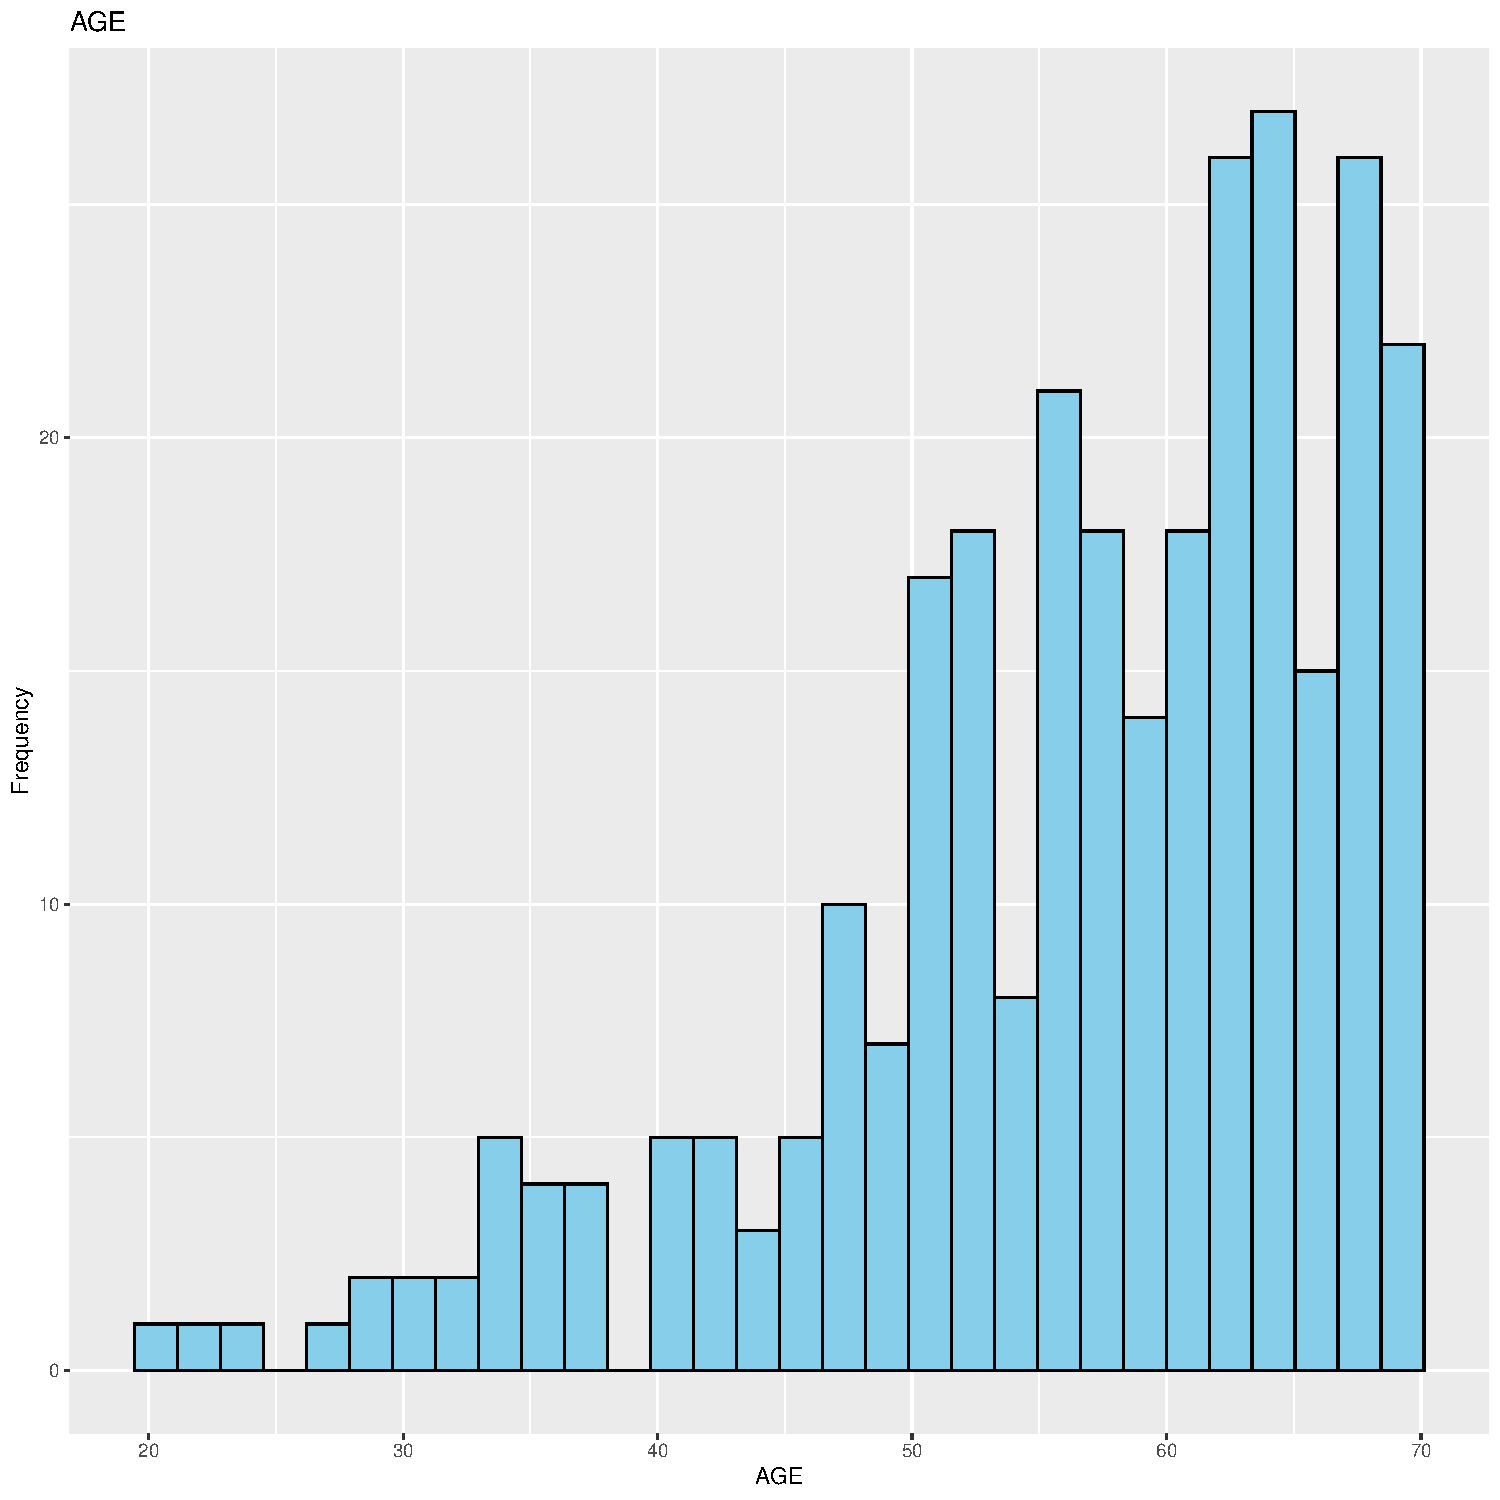
\includegraphics[width=\columnwidth]{figures/clinical_data_var_dist/AGE}
	\caption{Age distribution histogram }
	\label{fig:ageDistrib}
\end{figure}

To now if the continuous variable were normally distributed, we used a Shapiro-Wilk test. The results showed that AGE, HGHT, BMI, TRISCHD all had p-value under 5\%, leading us to reject the null hypothesis, which say that the sample is drawn form a normally distributed population. However, for WGHT, it was higher than 5 , so we didn’t reject the null hypothesis (Table X ) . 

\begin{table}[H]
\begin{center}
	\setlength{\tabcolsep}{0.5pt}
	\begin{tabular}{ |c|c|c|c|c|c| } 
	\hline 
	& P-value   \\[0.2cm] 
	\hline
	 AGE &\small $1.14*10^{-11} $   \\ [0.1cm]
	\hline
	 HGHT &\small $2.38*10^{-05} $  \\[0.1cm]
	\hline
	 WGHT & \small $ 0.22 $  \\[0.1cm]
	\hline
	 BMI &   \small $6.54*10^{-05}  $ \\[0.1cm]
	\hline
	 TRISCHD &\small $7.70*10^{-11}$ \\[0.1cm]
	\hline
	 
\end{tabular}
\end{center}
\caption{Result of the Shapiro-Willk test on the continuous variables after rank-based inverse normal transformation (INT) }
\label{tab:swInt}
\end{table}






To do further analysis, we need them to be normally distributed. We tried to apply various transformations like log, square root, square. Only the square transformation successfully normalized the AGE sample. 
Because we needed it to work on all the continuous variable, we finally chose to use the rank-based inverse normal transformation (INT) (Table X)  . that first convert the variable into ranks, then map it to a normal distribution. 
\\

$ Y^t_{i}=  \Phi^{-1}(r-C/N-2C+1) $
\\

where $r_i$ is the ordinary rank of the $_ith$ case among the N observations and $\Phi^{-1}$ denotes the standard normal quantile (or probit) function.For the value of C we use C=3/8 \citep{beasley2009rank}.

\begin{table}[H]
\begin{center}
	\setlength{\tabcolsep}{0.5pt}
	\begin{tabular}{ |c|c|c|c|c|c| } 
	\hline 
	& P-value   \\[0.2cm] 
	\hline
	 AGE &\small $0.11 $   \\ [0.1cm]
	\hline
	 HGHT & \small $0.063 $ \\[0.1cm]
	\hline
	 WGHT & \small $ 1 $   \\[0.1cm]
	\hline
	 BMI &  \small $1 $\\[0.1cm]
	\hline
	 TRISCHD &\small $1$  \\[0.1cm]
	\hline
	 
\end{tabular}
\end{center}
\caption{Result of the Shapiro-Willk test on the continuous variables after rank-based inverse normal transformation (INT) }
\label{tab:swInt2}
\end{table}


If we look at the discrete variable, we can see that we don't have a balanced distribution. For example, for the variable SEX, there are more than twice as many males as females (fig x). For DTHHRDY, we can observe that most of the deaths occurred in ventilator cases (fig x). When conducting analysis, it's essential to keep these observations in mind as they can significantly influence the interpretation. 

\begin{figure}[H]
	\centering
	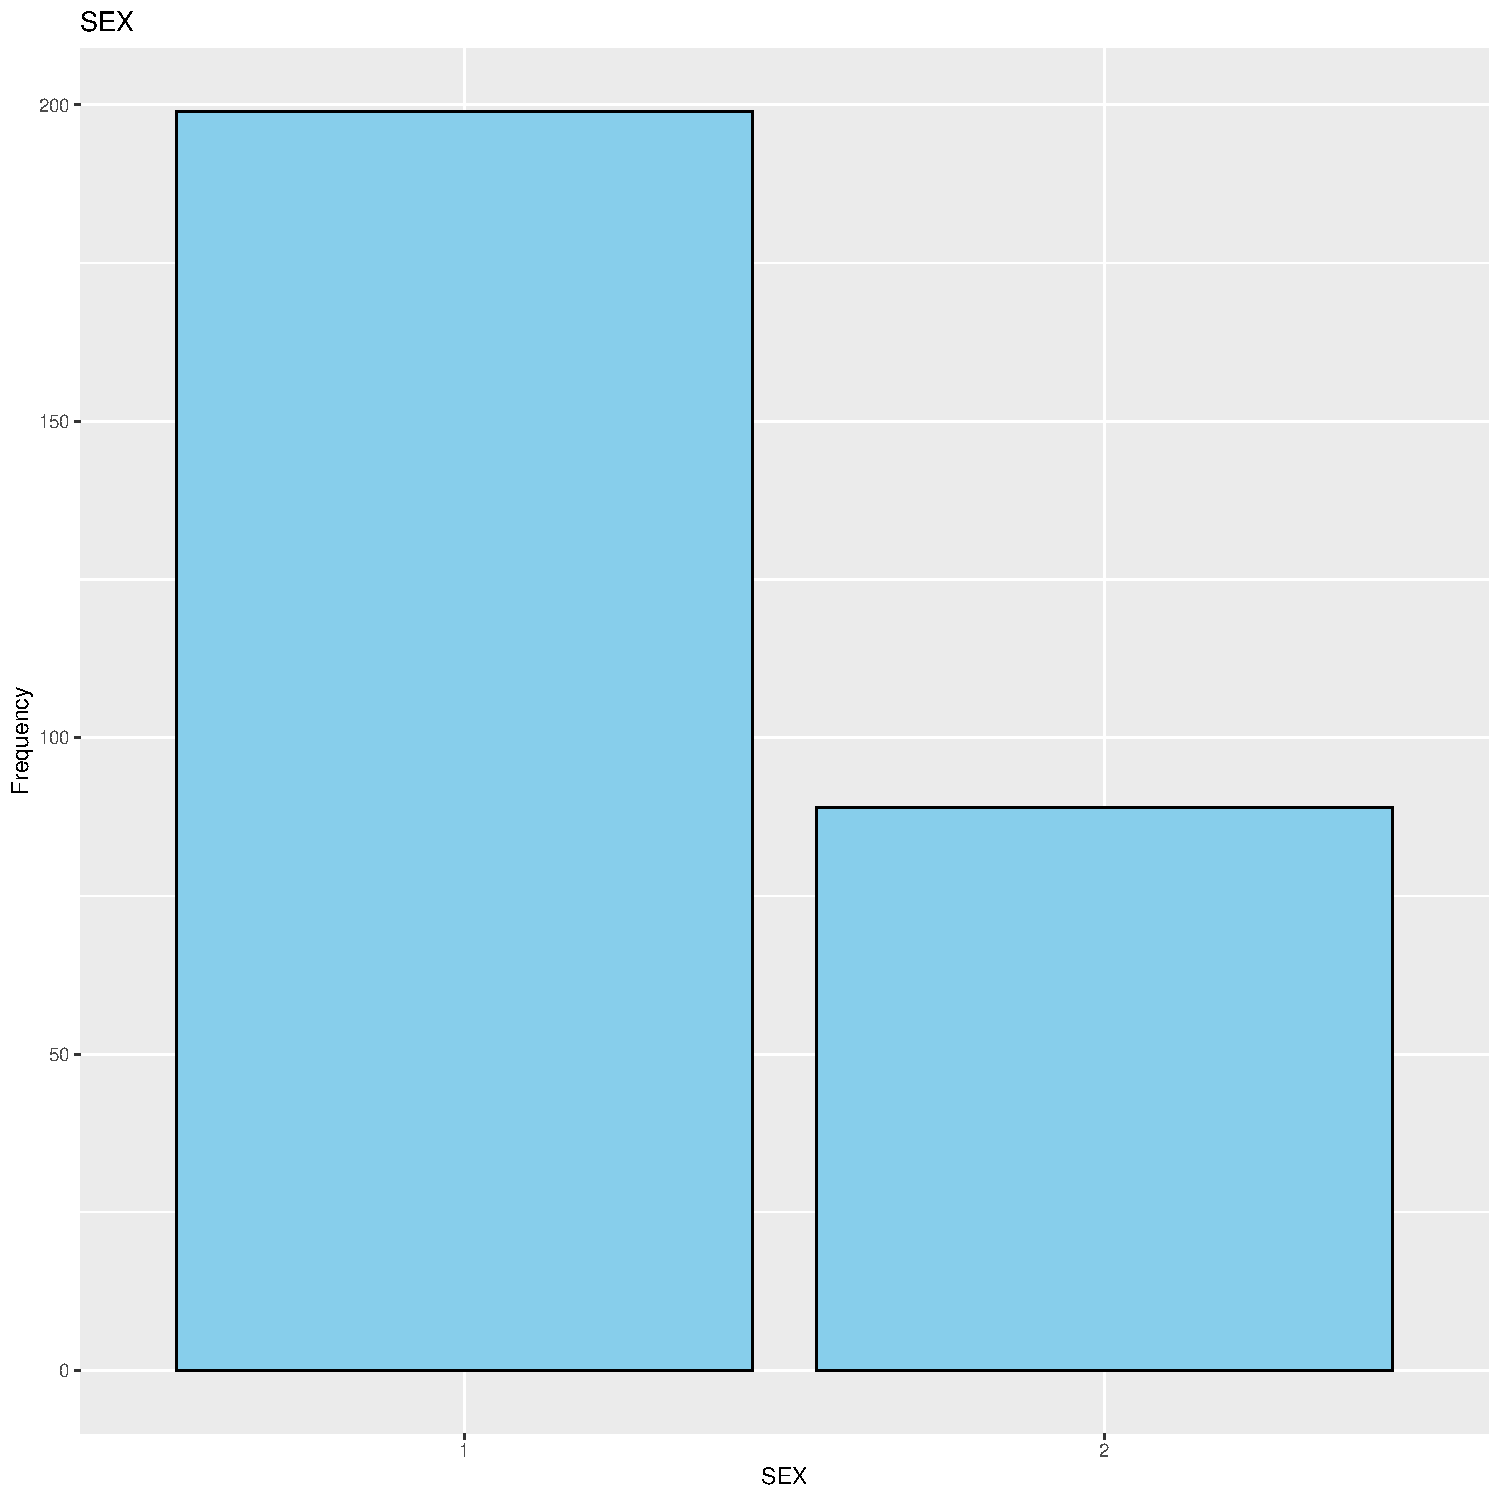
\includegraphics[width=\columnwidth]{figures/clinical_data_var_dist/SEX}
	\caption{SEX distribution histogram }
	\label{fig:sexDistrib}
\end{figure}

\begin{figure}[H]
	\centering
	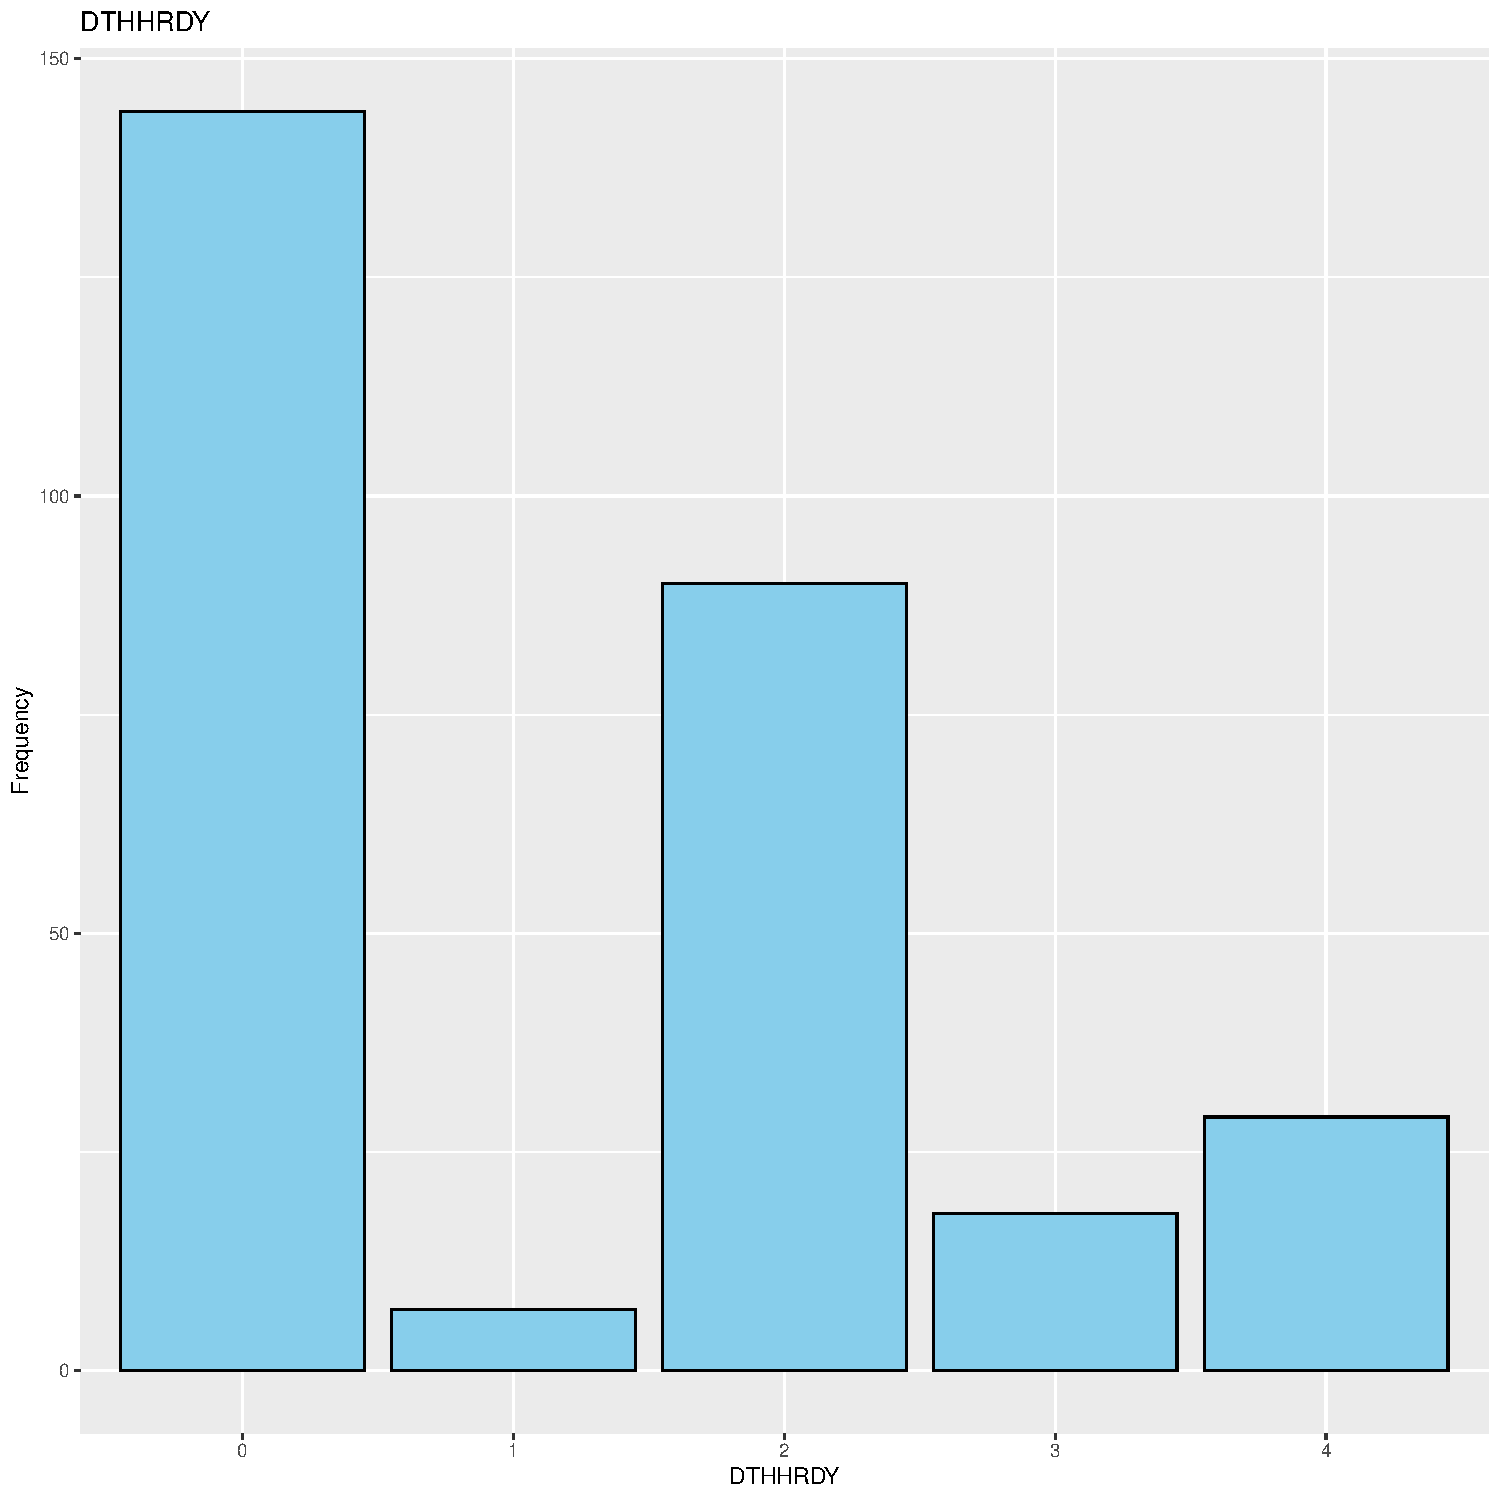
\includegraphics[width=\columnwidth]{figures/clinical_data_var_dist/DTHHRDY}
	\caption{DTHHRDY distribution histogram }
	\label{fig:dthhrdyDistrib}
\end{figure}

\subsection{Correlations between the clinical variables}

Principal Component Analysis (PCA) is a method of determining individual profiles and linear relationships between variables, based on correlation coefficients. The various graphs produced by a PCA, notably the correlation circle, are therefore a good way of illustrating the links between different quantitative variables, and getting a general idea of these links. Nevertheless, the data we are considering here are also partly qualitative. It is therefore preferable to turn to a Factor Analysis of Mixed Data, i.e. an analysis that applies a PCA to quantitative variables and a Multiple Correspondence Analysis to qualitative variables. The various dimensions defined by this method can be used to characterize all the variables. The FAMD() function in the FactoMineR package was used, with the argument allowing the creation of a series of graphs.

\begin{figure}[H]
	\centering
	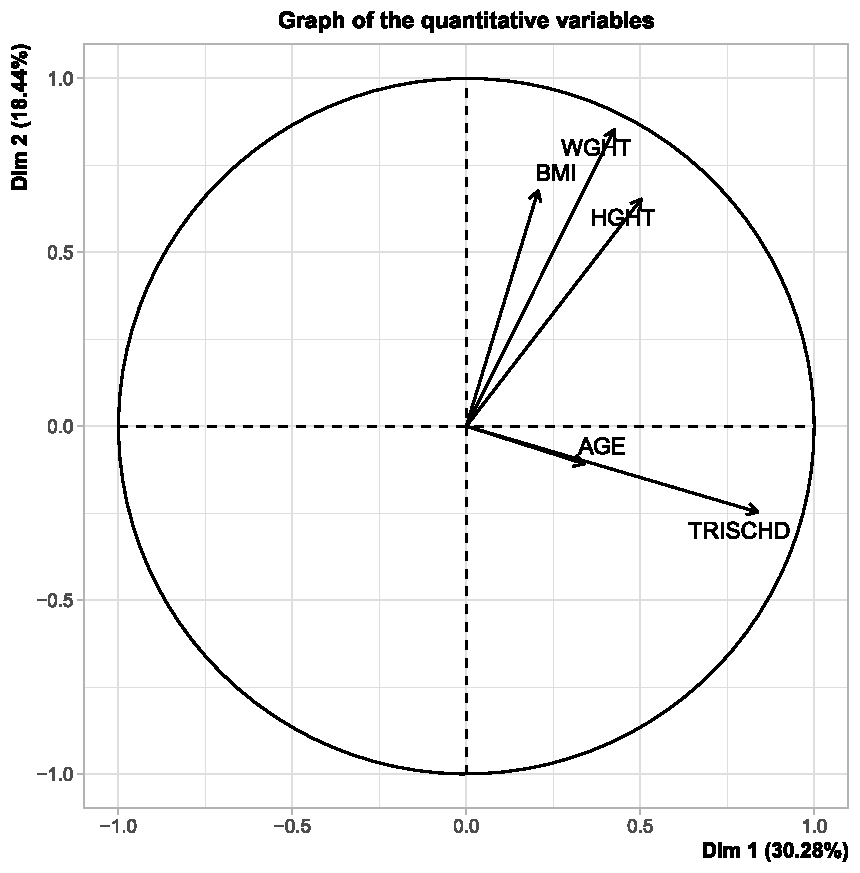
\includegraphics[width=\columnwidth]{figures/clinical_correlation_plots/all_quant_Dim2}
	\caption{Correlation circle of the continuous variables}
	\label{fig:corCircle}
\end{figure}

\begin{figure}[H]
	\centering
	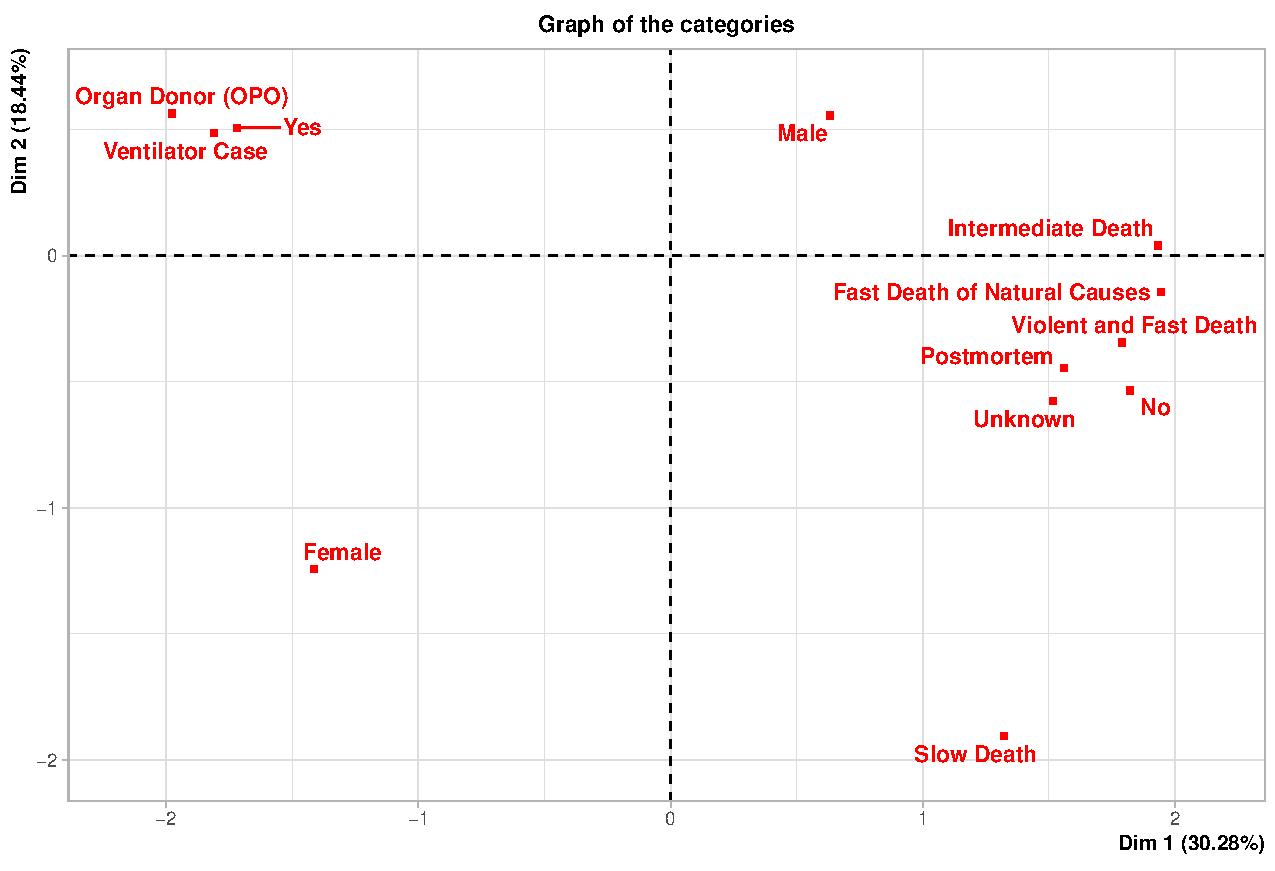
\includegraphics[width=\columnwidth]{figures/clinical_correlation_plots/all_categ_Dim}
	\caption{Level maps of all the different categories in the qualitative variables}
	\label{fig:lvlMap}
\end{figure}

The correlation circle allows us to represent quantitative variables according to the relationships they might have with each other, and the degree of explanation of these variables provided by the chosen dimensions. 
In this case, the two dimensions represented together explain only 48.72\% of the data, suggesting a certain complexity. 
This graph shows some correlation between the variables height (HGHT), weight (WGHT) and body mass index (BMI), which is not surprising given that taller people tend to be heavier, and also given that BMI is a function of height and weight. 
There also appears to be a correlation between age (AGE) and ischemic time (TRISCHD), i.e. the time between an individual's death and organ removal. 
This last observation is more difficult to explain intuitively. 
We can, however, point out that the variable AGE is weakly explained by the first two dimensions chosen, since its vector is close to the origin. 
This indicates that this possible correlation may not be significant, since by considering other dimensions, the vectors could be significantly far apart.

In contrast to the correlation circle, the level map represents the different categories or levels of categorical variables. 
We can already see that gender is close to different clusters. 
It would seem that there is a correlation between gender and type of death in these data, given that women seem to be more prone to ventilatory problems than men, which would explain the presence of a respirator before the person's death (Yes). 
It also appears that women are more likely than men to be organ donors. This graph therefore shows a certain correlation between gender and organ donation, type of death, but also between type of death and the presence or absence of a respiratory system prior to death.

Although these graphs illustrate the presence of possible correlations, they do not give any indication of their intensity, as they are not quantified. 
This quantification of correlation is particularly complex, as there is no correlation coefficient that can be applied to either quantitative or qualitative variables, or between these two types of variable. 
It was therefore decided to use different coefficients depending on the type of comparison, although this choice does not allow all correlations to be compared with each other. 
Correlations between quantitative variables were established using the cor() function with Spearman's method. 
This correlation was chosen because it does not require normally distributed variables, which is not the case for most of the variables considered. 
This coefficient is the only one to consider negative correlations.
Cramer's V was used to determine correlations between categorical variables, a coefficient based on the Chi-square statistic, and which is non-parametric. 
This correlation was calculated using the cramerV() function in the rcompanion package, with a bias correction given that this test tends to overestimate the relationships between categorical variables.
Logistic regression is used to determine the correlation between a quantitative variable and a binomial categorical variable, in this case gender and cohort. 
Finally, Cramer's V is applied to the H statistic of the Kruskall-Willis test between categorical and quantitative variables, as this statistic is the Kruskall-Willis chi-square. This application simply involves calculating the square root of the H statistic divided by the number of observations, the H statistic coming from the kruskall.willis() function.

\begin{figure}[H]
	\centering
	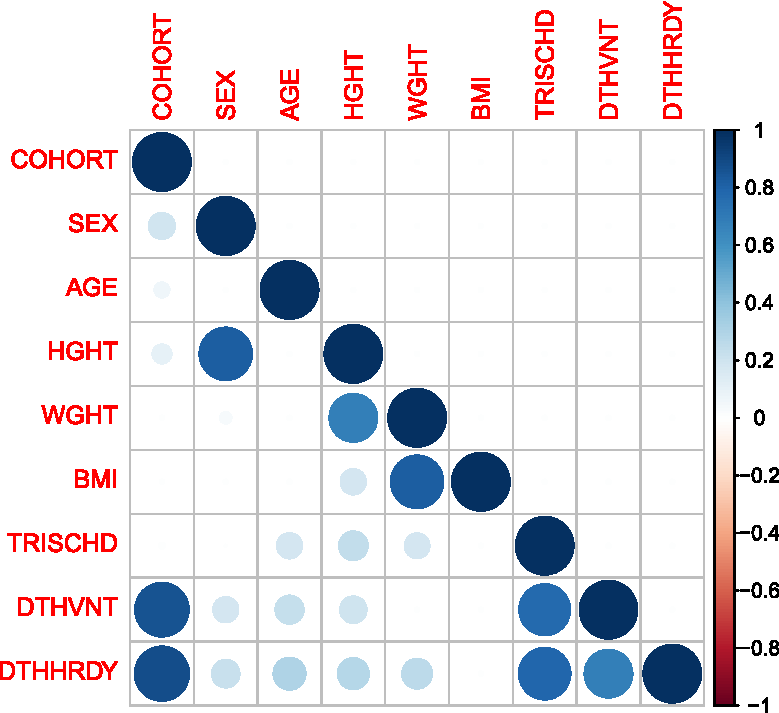
\includegraphics[width=\columnwidth]{figures/clinical_correlation_plots/corrected_allCorrelations2}
	\caption{Correlation matrix of all the variables}
	\label{fig:allCor}
\end{figure}

Looking at all the results together, we can see that there is a significant correlation between gender and height, which can simply be explained by the fact that men are generally taller than women. 
The correlation between height and weight, as well as between weight and BMI, can be explained as described above. 
Nevertheless, the absence of any significant correlation between height and BMI is rather odd given that the BMI calculation takes into account both height and weight, and that the correlation circle has positioned the corresponding vectors relatively close to each other. 
There is also a correlation between cohort and both type of death (DTHHRDY) and use of artificial ventilation before death (DTHVNT). 
There is a certain logic behind these correlations: the cohort variable divides people into organ donors and postmortem donors, i.e. victims of brain or cardiac death, thus depending on the type of death, but we can also consider that people with brain death are generally assisted with artificial ventilation before death. 
There also seems to be a correlation between the time between the individual's death and the removal of his or her organs and the type of death, but also the presence of a ventilatory apparatus. 
Finally, DTHVNT and DTHHRDY are also correlated.

\begin{table*}[t]
\footnotesize
\makebox[\linewidth]{
\begin{tabular}{|c|c c|c|c c|c c|c c|c|c c|c|cc|}
\cline{2-8}
    \hline & \multicolumn{2}{c|}{\rotatebox{90}{AGE}} & \rotatebox{90}{SEX} & \multicolumn{2}{c|}{\rotatebox{90}{HGHT}} & \multicolumn{2}{c|}{\rotatebox{90}{WGHT}} & \multicolumn{2}{c|}{\rotatebox{90}{BMI}} & \rotatebox{90}{COHORT} & \multicolumn{2}{c|}{\rotatebox{90}{TRISCHD}} & \rotatebox{90}{DTHVNT} & \multicolumn{2}{c|}{\rotatebox{90}{DTHHRDY}} \\
    \hline 
\rotatebox{90}{Cluster} &
  \rotatebox{90}{Normalized} &
  \rotatebox{90}{Categorical (56+ vs -56)} &
  \rotatebox{90}{Female vs Male} &
  \rotatebox{90}{Normalized} &
  \rotatebox{90}{Categorical (71+ vs -71)} &
  \rotatebox{90}{Normalized} &
  \rotatebox{90}{Categorical (181+ vs -181)} &
  \rotatebox{90}{Normalized} &
  \rotatebox{90}{Categorical (28+ vs -28)} &
  \rotatebox{90}{PostMortem vs OrganDonor} &
  \rotatebox{90}{Normalized} &
  \rotatebox{90}{Categorical (50+ vs -50)} &
  \rotatebox{90}{Yes vs No} &
  \rotatebox{90}{Intermediate vs Slow} &
  \rotatebox{90}{Fast vs Slow} \\
  \hline
0 &  & \cellcolor[HTML]{FDFF89}1,22 & \cellcolor[HTML]{B4F5F2}-1,26 &  &  &  &  &  &  & \cellcolor[HTML]{FDFF89}1,98 &  & \cellcolor[HTML]{FDFF89}1,78 & \cellcolor[HTML]{B4F5F2}-1,49 & \cellcolor[HTML]{FDFF89}2,10 & \cellcolor[HTML]{FDFF89}2,00 \\
1 &  &  &  &  &  &  &  &  &  &  &  &  &  &  &  \\
2 &  & \cellcolor[HTML]{FDFF89}1,87 & \cellcolor[HTML]{B4F5F2}-1,99 &  &  &  & \cellcolor[HTML]{FDFF89}1,15 &  & \cellcolor[HTML]{FDFF89}1,70 & \cellcolor[HTML]{FDFF89}2,46 &  & \cellcolor[HTML]{FDFF89}2,36 & \cellcolor[HTML]{B4F5F2}-2,38 & \cellcolor[HTML]{FDFF89}1,71 & \cellcolor[HTML]{FFC702}2,85 \\
3 &  &  &  &  &  &  &  &  &  & \cellcolor[HTML]{FDFF89}1,24 &  &  &  &  &  \\
4 &  &  &  &  &  &  &  &  &  &  &  &  &  &  &  \\
5 &  &  &  &  &  &  &  &  &  & \cellcolor[HTML]{FDFF89}1,55 &  & \cellcolor[HTML]{FDFF89}1,19 & \cellcolor[HTML]{B4F5F2}-1,41 &  &  \\
6 &  &  & \cellcolor[HTML]{FDFF89}1,70 & \cellcolor[HTML]{B4F5F2}-1,02 & \cellcolor[HTML]{B4F5F2}-2,32 &  &  &  &  & \cellcolor[HTML]{6F94FF}-5,33 &  & \cellcolor[HTML]{6F94FF}-5,91 & \cellcolor[HTML]{F56B00}6,27 & \cellcolor[HTML]{6F94FF}-6,34 & \cellcolor[HTML]{6F94FF}-5,90 \\
7 &  &  &  &  &  &  &  &  &  & \cellcolor[HTML]{B4F5F2}-1,10 &  &  &  &  &  \\
8 &  &  & \cellcolor[HTML]{FDFF89}1,03 &  &  &  &  &  &  & \cellcolor[HTML]{B4F5F2}-2,31 &  & \cellcolor[HTML]{B4F5F2}-2,02 & \cellcolor[HTML]{FDFF89}2,17 & \cellcolor[HTML]{B4F5F2}-2,25 & \cellcolor[HTML]{B4F5F2}-2,02 \\
9 &  &  &  &  &  &  &  &  &  & \cellcolor[HTML]{FDFF89}1,17 &  &  &  &  &  \\
10 &  & \cellcolor[HTML]{B4F5F2}-1,53 & \cellcolor[HTML]{FDFF89}1,07 &  & \cellcolor[HTML]{4AD7FF}-2,69 &  & \cellcolor[HTML]{4AD7FF}-2,60 &  &  & \cellcolor[HTML]{6F94FF}-6,72 & \cellcolor[HTML]{B4F5F2}-1,12 & \cellcolor[HTML]{6F94FF}-6,90 & \cellcolor[HTML]{F56B00}7,35 & \cellcolor[HTML]{6F94FF}-6,41 & \cellcolor[HTML]{6F94FF}-7,12 \\
11 &  &  &  &  &  &  &  &  &  &  &  &  &  &  &  \\
12 &  &  &  &  &  &  &  &  &  & \cellcolor[HTML]{B4F5F2}-1,32 &  &  & \cellcolor[HTML]{FDFF89}1,03 &  &  \\
13 &  &  &  &  &  &  &  &  &  &  &  &  &  &  &  \\
14 &  &  &  &  &  &  &  &  &  & \cellcolor[HTML]{B4F5F2}-1,84 &  & \cellcolor[HTML]{B4F5F2}-1,72 & \cellcolor[HTML]{FDFF89}1,78 & \cellcolor[HTML]{B4F5F2}-1,62 & \cellcolor[HTML]{B4F5F2}-1,58 \\
15 &  &  &  &  &  &  &  &  &  & \cellcolor[HTML]{FDFF89}1,25 &  & \cellcolor[HTML]{FDFF89}1,04 & \cellcolor[HTML]{B4F5F2}-1,03 &  &  \\
16 &  &  &  &  &  &  &  &  &  & \cellcolor[HTML]{FDFF89}1,48 &  & \cellcolor[HTML]{FDFF89}1,19 & \cellcolor[HTML]{B4F5F2}-1,07 & \cellcolor[HTML]{FDFF89}1,41 &  \\
17 &  &  &  &  &  &  &  &  &  & \cellcolor[HTML]{B4F5F2}-1,42 &  &  &  &  & \cellcolor[HTML]{B4F5F2}-1,20 \\
18 &  &  &  &  &  & \cellcolor[HTML]{FFC702}4,40 &  & \cellcolor[HTML]{FFC702}3,12 &  &  & \cellcolor[HTML]{6F94FF}-5,25 &  &  &  &  \\
19 &  &  &  &  &  &  &  &  &  &  &  &  &  &  &  \\
20 &  &  & \cellcolor[HTML]{FDFF89}1,02 &  &  &  &  &  &  & \cellcolor[HTML]{B4F5F2}-2,38 &  & \cellcolor[HTML]{B4F5F2}-2,07 & \cellcolor[HTML]{FDFF89}2,44 & \cellcolor[HTML]{B4F5F2}-2,43 & \cellcolor[HTML]{B4F5F2}-2,26 \\
21 &  &  & \cellcolor[HTML]{B4F5F2}-1,09 &  &  &  &  &  &  & \cellcolor[HTML]{FDFF89}1,83 &  & \cellcolor[HTML]{FDFF89}1,60 & \cellcolor[HTML]{B4F5F2}-1,69 & \cellcolor[HTML]{FDFF89}1,68 & \cellcolor[HTML]{FDFF89}1,73 \\
22 &  &  &  &  &  &  &  &  &  & \cellcolor[HTML]{FDFF89}1,47 &  & \cellcolor[HTML]{FDFF89}1,22 & \cellcolor[HTML]{B4F5F2}-1,26 & \cellcolor[HTML]{FDFF89}1,23 & \cellcolor[HTML]{FDFF89}1,02 \\
23 &  &  & \cellcolor[HTML]{FDFF89}1,28 &  & \cellcolor[HTML]{B4F5F2}-1,56 &  &  &  &  & \cellcolor[HTML]{4AD7FF}-4,53 &  & \cellcolor[HTML]{4AD7FF}-4,22 & \cellcolor[HTML]{F56B00}5,19 & \cellcolor[HTML]{6F94FF}-5,27 & \cellcolor[HTML]{4AD7FF}-4,91 \\
24 &  &  &  &  &  &  &  &  &  & \cellcolor[HTML]{FDFF89}2,19 &  & \cellcolor[HTML]{FDFF89}1,93 & \cellcolor[HTML]{B4F5F2}-1,61 & \cellcolor[HTML]{FDFF89}2,22 & \cellcolor[HTML]{FDFF89}2,09 \\
25 &  &  & \cellcolor[HTML]{FDFF89}1,59 &  & \cellcolor[HTML]{B4F5F2}-1,42 &  &  &  &  & \cellcolor[HTML]{6F94FF}-5,75 &  & \cellcolor[HTML]{6F94FF}-5,21 & \cellcolor[HTML]{F56B00}5,58 & \cellcolor[HTML]{6F94FF}-6,35 & \cellcolor[HTML]{6F94FF}-5,25 \\
26 &  &  &  &  &  &  &  &  &  & \cellcolor[HTML]{FDFF89}1,72 &  & \cellcolor[HTML]{FDFF89}1,17 & \cellcolor[HTML]{B4F5F2}-1,46 & \cellcolor[HTML]{FDFF89}1,28 & \cellcolor[HTML]{FDFF89}1,57 \\
27 &  &  &  &  & \cellcolor[HTML]{B4F5F2}-1,14 &  &  &  &  & \cellcolor[HTML]{4AD7FF}-3,09 &  & \cellcolor[HTML]{4AD7FF}-2,62 & \cellcolor[HTML]{FFC702}2,92 & \cellcolor[HTML]{4AD7FF}-3,27 & \cellcolor[HTML]{4AD7FF}-2,85 \\
28 &  &  &  &  &  &  &  &  &  &  &  &  &  &  &  \\
29 &  &  &  &  &  &  &  &  &  &  &  &  &  &  &  \\
30 &  &  &  &  &  &  &  &  &  &  &  &  &  &  &  \\
31 &  & \cellcolor[HTML]{B4F5F2}-1,57 &  &  & \cellcolor[HTML]{B4F5F2}-1,47 &  & \cellcolor[HTML]{B4F5F2}-1,72 &  & \cellcolor[HTML]{B4F5F2}-1,10 & \cellcolor[HTML]{4AD7FF}-4,27 & \cellcolor[HTML]{B4F5F2}-1,38 & \cellcolor[HTML]{4AD7FF}-4,64 & \cellcolor[HTML]{F56B00}5,01 & \cellcolor[HTML]{6F94FF}-5,77 & \cellcolor[HTML]{4AD7FF}-4,42 \\
\hline
\end{tabular}}
\caption{Significant fold changes for each variable considered in this project, we also considered to categorize the continous data as a possible way to have more significant results.}
\label{tab:Q2FC}
\end{table*}

\subsection{Impact of technical variables on clinical variables}

In this section, we investigate the influence of technical variables on clinical data and describe the methodology employed to isolate their effects.
To decouple the impact of technical variables from the data of interest, linear regression analyses were conducted.
Prior to regression, the data underwent transformation using inverse data normalization for numerical variables (cf. section 1.1).

From the preceding section where correlations between variables were examined, certain expectations were established.
Age was anticipated to be associated with TRISCHD, DTHHRDY, and COHORT, while height and weight were expected to be linked to the same variables.
Additionally, sex appeared correlated with DTHHRDY and COHORT. Surprisingly, BMI seemed uncorrelated with any technical variables.

For the technical variable DTHHRDY, a decision was made to group the categories into three new categories: slow, intermediate, and fast.
This choice was made since more observations by categories would enhance statistical power.

Upon conducting linear regression (generalized linear regression in the case of the categorical variable sex), it was observed that age was dependent on cohort, sex was dependent on DTHHRDY, height was dependent on DTHHRDY, weight was dependent on DTHHRDY, and, surprisingly, BMI was dependent on both DTHHRDY and COHORT.

Subsequently, linear regression (or generalize d linear regression) was rerun for each variable of interest, utilizing only the significant technical variables from the overall models.
The residuals of these models were stored for further analysis.
These residuals represent the data of interest with the unwanted effects of the technical variables removed, providing a clearer understanding of the clinical data.

As we we will see in a next section, we decided to not use the residuals for the differential expression analysis. This is because the method used (DESeq2 \citep{DESeq2:2014}), allow to use the technical variables as a contrast in the design of the analysis. By doing that we can adjust the analysis to take into account the confonding effect of the technical variables.

\section{Association between clinical variables and morphological data}

\subsection{Method}

To investigate the relationship between clinical and morphological data, we treated this problem as a differential expression analysis. 
In this case, the clinical data represents the samples metadata and the morphological data the features. 
This approach allow us to take advantage of the numerous tools and methods developed for differential expression analysis.
Here we used the DEseq2 package \citep{DESeq2:2014}. The strength of DESeq2 is that it does correct the morphological count matrix to take into account potential bias. 
These bias are for instance the difference in the total count between samples and the difference in library composition that can lead to bad normalisation if not taken into account. 
To execute this normalisation, DESeq2 will compute geometric mean for each morphological cluster. 
Then, it will use these values and create a new matrix that consists of the counts divided by their associated geometric mean. 
After that it will use this new matrix to build scaling factors for each sample, and finally applying this scaling factor to the original counts.

(Add pval test)

For the question 2.1 and 2.2 we used the each clinical variable and each technical variable as the contrast for the design of the differential analysis.
For the question 2.3 we used a contrast composed of each clinical variable plus the technical variables that were significantly associated with the clinical variable in the previous section.
By doing that we ensure that we adjust the analysis to take into account the confonding effect of the technical variables.
Note that for numerical variables, we used the rank-based inverse normal transformated values obtained in the Question 1.1.

We also decided to make extra analysis by converting the numeric clinical data to binary data. By doing this we assume to obtain more significant results. 
This can be explained by the fact that the DESeq2 method will in the case of continous variable report the log2 fold change per unit of change of that variable.
Therefore for variables with an high range of value, the fold change will be very low. By using binary variable we can increase the fold change and therefore the significance of the results.
The binary conversion was done by taking the median of the variable as the threshold to separate the two categories.

Some other changes have been made for this analysis, they are listed in the following:
\begin{itemize}
	\item  The Hardy scale variable was converted to an 3 categories variable, by grouping the intermediate and slow categories together (cf. Q1)
	\item  Samples with DTHVNT unknown were discarded
	\item  A pseudo-count of 1 was added to the count matrix to avoid log transformation of 0 values
\end{itemize}


As for the interpretation of the results, we decided to fix the threshold values as follow, alpha at 0.05 and log2 fold change at 1.


\subsection{Clinical data vs. morphological data}

As a reminder, the clinical variables correspond to AGE, SEX, HGHT, WGHT and BMI. The results of the association of these variables with morphological clusters therefore correspond to the first five columns of Table \ref{tab:Q2FC}.
For the AGE variable, we can see that there are no significant results, no fold change, simply by considering the standardized values of this variable. Nevertheless, by dividing these values into two age groups of over and under 56, we can observe 4 clusters with significant characteristics. Clusters 0 and 2 have positive fold change values, indicating that these two clusters are made up of parts of samples from donors aged over 56, unlike clusters 10 and 31. 

In terms of sex, clusters 0, 2 and 21 have negative values, indicating a greater representation of male donors in these clusters, in contrast to clusters 6, 8, 10, 20, 23 and 25. It should be noted, however, that a relatively large number of clusters are characterized by females, even though these represent a certain minority of the data used. 

With normalized values for individual height, only cluster 6 shows a fold change whose negative value seems to indicate a certain number of shorter donors. This cluster is also repeated when we categorize this variable, but with a more pronounced fold change. We also find clusters 10, 23, 25, 27 and 31. All these clusters have a negative fold change for this categorized variable, indicating the presence of sample parts from relatively smaller donors, measuring less than 71 inch or 180cm. The term 'relatively' is important here, as the median is particularly high in this dataset.

According to the normalized values of individual weights, we only observe a particularly positive fold change for cluster 18, which disappears when we consider this variable categorically. This observation can be explained by the fact that, in the case of a continuous variable, the fold change should be considered as the increase in the number of tiles in a cluster as the values of the variable increase. In other words, the positive value for cluster 18 indicates that, as we consider values with increasingly large weights, the number of tiles corresponding to these weights will become larger and larger. Thus, cluster 18 comprises a smaller number of tiles from low-weight donors, and a larger number of tiles from higher-weight donors. The absence of this cluster in the categorical column may be explained by a rather even distribution of these weight values on either side of the median. This particularity of cluster 18 could also be explained by the fact that it contains very few tiles (32.4k) compared with the majority of clusters (more or less 200k). In the categorical part, cluster 2 seems to be made up preferentially of tiles from donors over 181 pounds, or 82.1 kg, unlike clusters 10 and 31.

The same observations regarding cluster 18 can be made with the BMI variable. Furthermore, once again, cluster 2 has a positive value indicating a greater presence of donors with a BMI of over 28, i.e. in obese or overweight conditions \citep{cdc_all_2022}, unlike cluster 31.

From a more global point of view, clusters 10 and 31 are particularly similar, and this similarity can be explained by the fact that they are very close to each other in the morphological atlas of the organ studied. As such, they have similar characteristics, as the different tiles that constitute them largely originate from the same anterior cluster (G3\_C1). The different results also underline the correlations determined previously, notably the correlation between sex and height, and between weight and BMI.

\subsection{Technical data vs. morphological data}

Technical variables include COHORT, TRISCHD, DTHVNT and DTHHRDY. Their associations with the various clusters are therefore shown in the last 4 columns of Table \ref{tab:Q2FC}. 

The COHORT variable represents the type of organ donor, and since we are comparing the post-mortem class with simple organ donors, positive values correspond to a higher proportion of tiles from post-mortem, brain-dead donors. Particularly negative values can be seen for clusters 6, 10, 23, 25, 27 and 31, indicating a particularly high proportion of classic organ donors.

Comparing normalized and categorized ischemic time, we can again see that cluster 18 returns a significant result in the former case, but not the latter. Following the same logic as above, we can assume that this cluster contains a significant proportion of tiles from organs with relatively low ischemic times, but that the distribution of these times within the cluster does not appear to differ significantly on either side of the overall median. Surprisingly, this kind of result only appears for cluster 18. Although a negative value here corresponds to an ischemic time of less than 50 minutes, and vice-versa for positive values.

As previously mentioned, the DTHVNT variable corresponds to the presence or absence of respiratory assistance prior to the patient's death. Since we are comparing the presence with the absence of such assistance, positive results correspond to a relative abundance of individuals with respiratory assistance in the cluster, and vice versa for negative values. A certain inverse relationship can be observed between the COHORT and DTHVNT variables: among common clusters, the results are of opposite signs, and the importance of these values is comparable. This observation can be explained by the fact that there is a correlation between these two variables. Comparison with the TRISCHD results, which are of opposite sign for common clusters, highlights the correlation that also exists between the two variables. 

The DTHHRDY variable contains the types of death, considered here as slow, intermediate and fast. The last two types are compared with slow death. We can see that the vast majority of clusters with a result for one comparison also return a result of the same sign for the other comparison. Thus, a double positive result implies that the cluster contains mainly tiles from people with relatively rapid or intermediate death, and by extension a very small amount of tiles from patients with slow death. Conversely, a double-negative result implies that the cluster is particularly characterized by slow deaths. Cluster 16, on the other hand, is characterized by intermediate death, and cluster 17 by only a low rate of rapid death. As before, these results also express correlations between DTHHRDY and the variables COHORT, TRISCHD and DTHVNT. 

Looking at all the values, several clusters stand out for their absolute fold change values for each technical variable, but also for the presence of certain patterns. For example, clusters 6, 10, 23, 25, 27 and 31 each have particularly negative values, except for the DTHVNT variable, which has very positive values. These similarities also appear in the morphological atlas, in terms of their position in relation to each other. We've already highlighted the fact that clusters 10 and 31 follow one another, but clusters 23, 27 and 6 also follow one another, but are simply separated by a different cluster. Since they are relatively close, we can assume that some of their similarities can be explained by tiles from previous clusters (G3) in common. Conversely, some clusters have positive values for all technical variables except DTHVNT, i.e. clusters 0, 2, 21, 22, 24 and 26. Their positions in the morpholigic atlas allow us to determine that their tiles come from common clusters, notably G3\_C7.

\subsection{Adjusted clinical data vs. morphological data}

The analysis was redone for non-technical variables to incorporate adjustments for confounding variables. The non-technical variables include AGE, SEX, HGHT, WGHT, and BMI. These variables were adjusted for variations  of the technicals variables found to be dependent on them (cf. section 2.3). 
Adjustments were applied only to categorized variables as they yielded more meaningful results.

Comparing Table 1 and Table 2, we observed significant changes. Initially, AGE displayed associations with 4 clusters. However, after adjustments, no clusters remained associated with AGE. This indicates that the clusters found in Table 1 were influenced by the confounding variable COHORT.
For SEX, initially, 9 clusters were associated. However, after adjustment, SEX showed no association with any cluster, suggesting that the associations observed previously were due to the influence of DTHHTRDY.

Regarding HGHT, adjustments reduced the number of associated clusters from 6 to 1(cluster 10). This cluster was the only one associated with HGHT, showing a log2 fold change of -1.32, indicating that it was 0.40 times less prevalent in individuals with a height over 71 pounds . 

For WGHT, while initially, 3 clusters were associated, after adjustment, these associations disappeared, and 3 other clusters became associated. Cluster 6 was 0.49 times less prevalent in individuals with a weight over 181 pounds , with a log2 fold change of -1.02. Cluster 11 exhibited an even lower prevalence (0.38 times) with a log2 fold change of -1.41, while Cluster 27 was 2.09 times more prevalent in this group, with a log2 fold change of 1.07.

Lastly, for BMI, initially 2 clusters were associated. However, after adjustment, no clusters remained associated. 



\section{Association between morphological data and gene expression}
\subsection{Association analyses at the level of the transcript}

We performed a differential gene expression analysis to identify significant up-regulated and down-regulated genes associated with each morphological cluster. Using the DESeq2 method, the analysis was carried out for each cluster, considering both the presence and absence of technical variable corrections. 

Differential analysis was conducted for each of the 32 clusters to determine the transcripts that varied significantly in function of the clusters.


To verify our results, an additional differential analysis was performed correcting for potential confounding effects of technical variables.

The following criteria where used to determine the significance of the results:
\begin{itemize}
    \item Log2 Fold Change Threshold: A threshold of 1 was set to consider significant changes in gene expression.
    \item Adjusted P-value Threshold: P-values were adjusted for multiple comparisons using Bonferroni correction. With 32 clusters, the adjusted significance threshold was set at 0.05/32.
\end{itemize}

For each cluster, we report the following:
\begin{itemize}
    \item Number of significant up-regulated and down-regulated genes, identified based on the set thresholds.
    \item Top 10 most significant up-regulated genes, ranked by the adjusted p-value.
\end{itemize}

\subsection{Gene Set Enrichment Analysis}
GSEA (Gene Set Enrichment Analysis) is a preranked method used to analyze gene expression data, allowing us to determine if genes within a given gene set exhibit non-random behavior. However, this method can be slow because the analytical form of the null distribution for the Enrichment Score (ES) statistic is not known, necessitating the calculation of an empirical null distribution.
The process involves calculating an ES value for each pathway. ES score are calculated by walking down the list of the ranked genes and increase a running-sum statistics if the gene is present in the set of gene for  a pathways and decreasing it if it is not present. The magnitude of the increase or decrease  depends of the correlation of the gene with the phenotype (\textcolor{red} {cluster ?}). The ES score of the pathways would be the running-sum statistics that is the farther from zero. 
Then generating random gene sets of the same size and calculating an ES for each of these random sets. .The P-value is estimated as the number of gene sets that have an ES value equals or more extreme and divided by the total number of generated random gene sets. But to have a good statistical power it needs a large number of gene set samples.

Here, we are going to use FGSEA (Fast Gene Set Enrichment Analysis), which efficiently estimates the GSEA P-value for a collection of pathways. It uses FGSEA-simple and FGSEA-multilevel on the pathways that have a low P-value.

FGSEA-simple calculates the estimated P-values efficiently and simultaneously for the whole collection of gene sets but with limited accuracy. It is based on the idea that random gene set samples can be shared between different input pathways. It estimates the P-value of a pathway with the largest gene set size “M” as a proportion of a sample of random gene sets of size KM, having the same or more extreme ES value as the pathway. For other pathways “j”, it constructs a set of independent samples of size Kj (Kj < KM) by considering the prefixes in each sample of the larger random gene set and then estimates the P-value using the set of independent samples. It also uses the idea that using the larger random gene sets, the ES values for all the prefixes can be calculated efficiently using a square root heuristic. It uses a variant of the enrichment curve where the enrichment curve is constructed starting with the gene that is the most up-regulated to the most down-regulated, with the curve going right if the gene is not present in the pathway and up if it is present. Then the enrichment score can be determined using the point that is furthest from the diagonal.

FGSEA-multilevel can estimate low P-values (P-value < $10{-6}$) accurately but for individual gene sets. It is based on a multilevel split Monte Carlo scheme. It calculates the probability of a random gene set of size K to have an enrichment score no less than $\gamma$, where $\gamma$ is an ES value > 0 given as input. Successively, the method finds ES levels ($l_i$) where the probability of ES being greater than the ES levels ($l_i$) is equal to $2^{-i}$. Finally, the method stops when $ l_i $becomes greater than $\gamma$ and when the P-value approaches $2^{-i}$.\citep{korotkevich2016fast}.

fgsea take as input a ranked list of or genes differentially expressed, we ranked them by significance and by the direction of the change using the formula:
\bigskip

 $ RANK =sign(FC)* -log_{10}(p-value)  $
 
\bigskip
Where FC is the log2(fold change).
We used this formula instead of the log2fold to take into account genes with a large fold change but non-significant and for p-value that are really small the gene can get a ranking of infinity. To get finite numbers we converted them to large or small values. By replacing the infinite values by 10 times the maximum or minimum ranking .
 At the top, we have the most significant and up-regulated genes, and at the bottom, the most significant down-regulated genes. Then it needs a list of gene sets. We used “c2.cp.reactome.v7.5.1.symbols.gmt”. This list of gene sets has been filtered to only contain genes  that are present in the ranked list of differentially expressed genes and with at least 5 genes present. Finaly, we run fgsea  \citep{fgsea} and exclude pathways that have gene set with a length under 10 and pathways with a gene set of over 1000 genes (\textcolor{red} {jutification ?}).
 
  For each cluster we repported the top  10 most significant up-regulated genes and top 10 most significant dow-regulated genes. The list has been order by NES by decreasing order, NES is the ES that has been normalized for each gene set to account for the differences of gene set size. 

\subsection{Technical and biological analysis}

From a purely numerical point of view, all clusters contain 102 significant genes, 47 of which are present in more than one cluster. However, when the confounding effects of technical variables are taken into account, these numbers fall to 82 significant genes for 24 genes common to several clusters. 

Among these common genes, ENSG00000215182.8 and ENSG00000223609.7 are present in 5 clusters, while ENSG00000095752.6, ENSG00000159261.10 and ENSG00000163435.15 are present in 4 clusters. Some of these genes are also found in common clusters, notably 11, 16, 21, 22, 23 and 26. But these similarities do not correspond to common morphological profiles, whether or not confounding effects are considered. 

\begin{figure}[H]
	\centering
	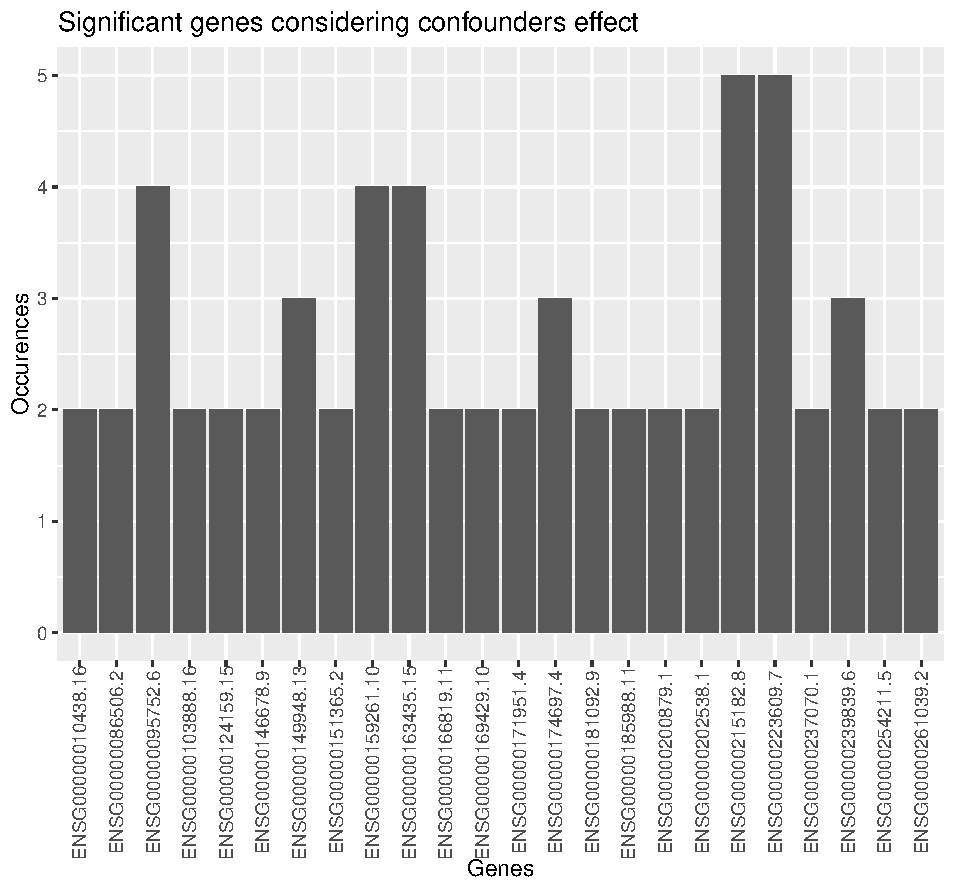
\includegraphics[width=\columnwidth]{figures/final_analysis/SigGenesConsideringConf}
	\caption{Genes present in at least 2 clusters, considering the confounder's effect}
	\label{fig:genesOcc}
\end{figure}

ENSG00000215182.8 corresponds to the MUC5AC gene encoding mucin-5AC, a glycoprotein that forms a gel mainly in gastric and respiratory epithelia. This gel protects the mucosa from infection and chemical damage in the gastric and respiratory tracts. This gene is also expressed in cardiac myxoma \citep{Islam2022}, a very common cardiac tumor corresponding to an abnormal mass of tissue. This tumor is biologically benign, but functionally malignant due to its position in the heart and the emboli it can generate  \citep{Chu2004}. This gene is up-regulated in clusters 3, 12, 16, 20 and 29, but they do not share common morphological profiles or similar death patterns. One might expect the presence of this gene to imply rapid deaths, since emboli can lead to relatively fulminant deaths, but the absence of this observation indicates that, for the majority of individuals considered, this myxoma was not the cause of their death. 

ENSG00000223609.7 is the HBD gene coding for the delta subunit of hemoglobin, a constituent of one type of erythrocyte. Expression of this gene in the heart may, at first glance, appear suspicious, since erythrocyte formation takes place mainly in the bone marrow. However, expression of this gene is also observed in various types of tissue, including cardyomyocytes  \citep{Keller2022}, the cardiac muscles that make up a very large part of the heart. The gene appears to be particularly expressed in clusters 0, 4, 11, 15 and 16, suggesting that these clusters are made up of a large number of cardiac muscle cells. 

ENSG00000095752.6 also designates the IL11 gene, coding for interleukin 11, a protein of the gp130 cytokine family. This cytokine stimulates the development of immunoglobulin-producing B cells in relation to T cells, thus playing a role in the induction of an immune response. The expression of this protein is also linked to a cardiac pathology, cardiac fibrosis, i.e. an accumulation of extracellular matrix to enable healing and tissue repair after some form of aggression. This pathology is not necessarily the main cause of organ dysfunction  \citep{Sweeney2023}. This gene is significantly expressed in clusters 3, 4, 17 and 29.

ENSG00000159261.10, better known as CLDN14, is a gene encoding claudin 14, a membrane protein that enables the formation of tight junctions between cells. This gene is expressed in clusters 3, 4, 16 and 28. Disconcertingly, clusters 4 and 16 are up-regulated for this gene and HBD, the latter indicating the presence of cardiac muscles, which do not have tight junctions  \citep{Severs1985}. Nevertheless, the presence of this type of intercellular junction may well be present in the heart, since it contains various epithelial tissues, such as the endocardium.

Finally, ENSG00000163435.15 corresponds to the ELF3 gene. This gene codes for E74 like ETS transcription factor 3, a transcription factor involved in the inflammatory response, up-regulation of transcription by RNA polymerase II. It's quite astonishing that this gene is particularly expressed in the heart, and what's more that it's among the 5 most present genes in the various clusters, since this gene shouldn't be expressed in the heart or that this expression is detectable. Indeed, it has been estimated that this gene is only detected in organs of epithelial origin, and it should be noted that the heart is of mesodermal origin. Nevertheless, this gene appears to be expressed in clusters 5, 11, 26 and 28.

\begin{figure}[H]
	\centering
	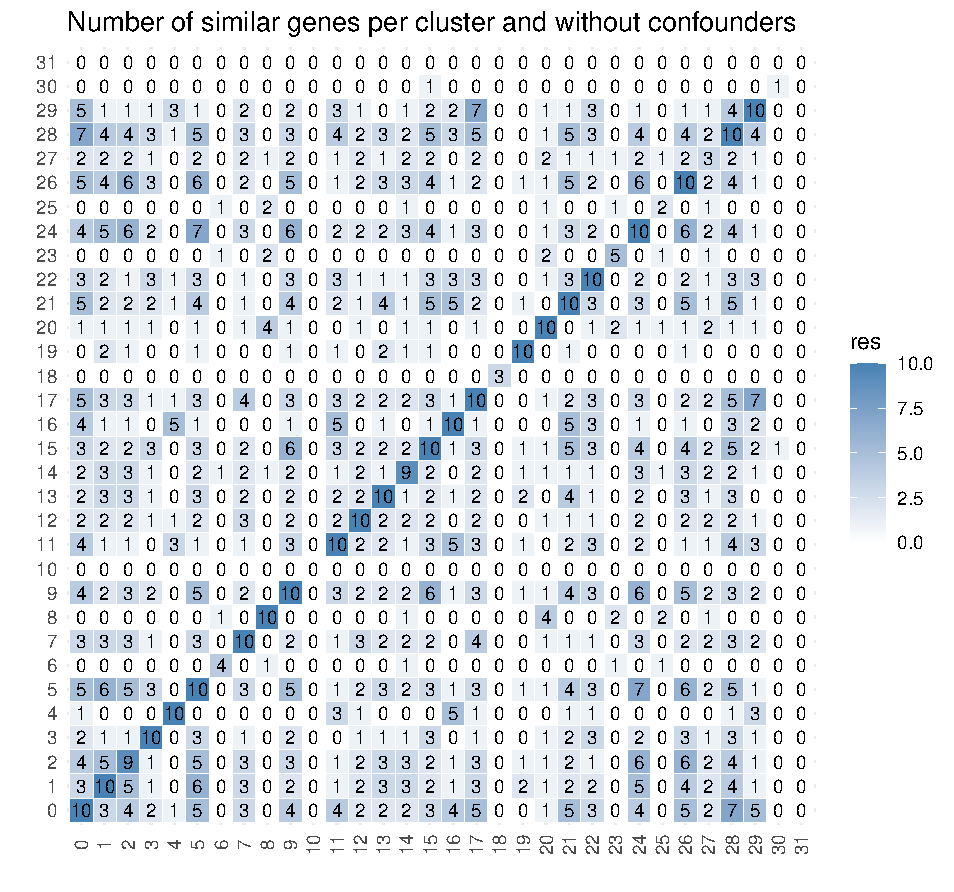
\includegraphics[width=\columnwidth]{figures/final_analysis/SimilGenes}
	\caption{Comparison of commun genes in the top 10 of all the clusters}
	\label{fig:similGenes}
\end{figure}


\begin{figure}[H]
	\centering
	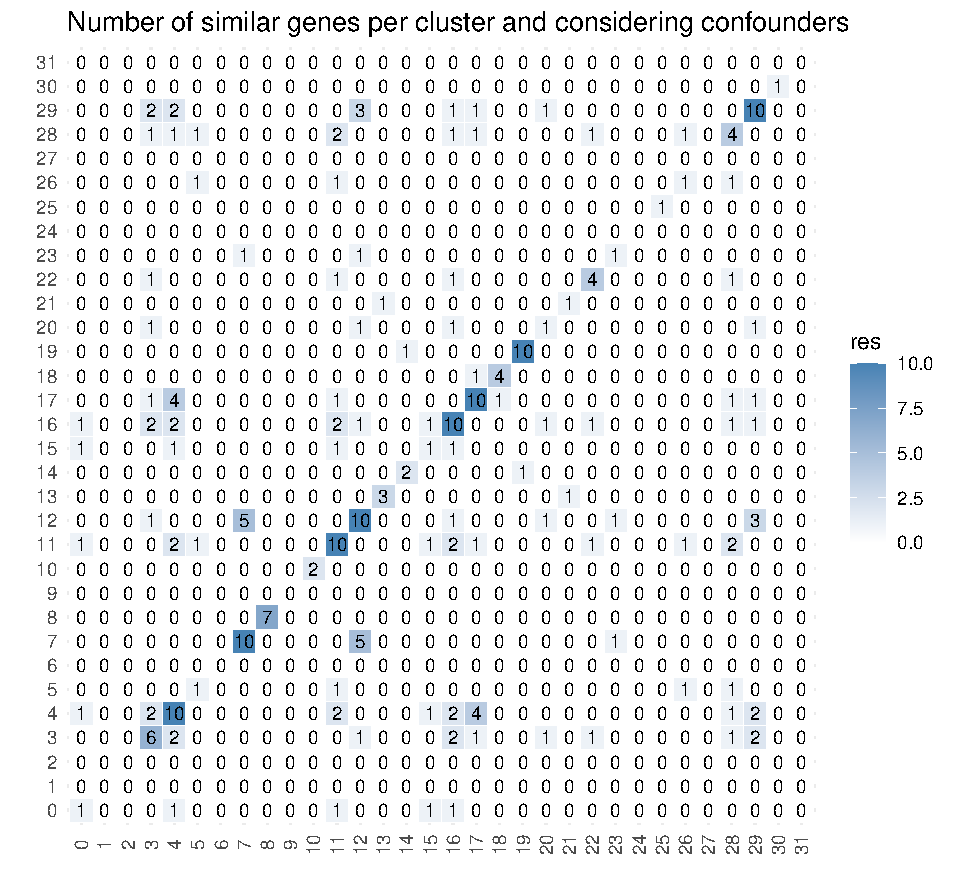
\includegraphics[width=\columnwidth]{figures/final_analysis/SimilConsideringConf}
	\caption{Comparison of commun genes in the top 10 of all the clusters, considering the confounder effect}
	\label{fig:similGenesConf}
\end{figure}

In addition to the biological analysis of these genes, it is also interesting to consider the number of significant genes in common between each cluster. First of all, we can see the importance of confounding effects, with a large number of similarities disappearing completely or decreasing drastically. One might also expect to observe the same patterns as in Table 1, since these results are also driven by clinical variables, but several examples demonstrate that this is not the case. Cluster 0 shares 7 genes with cluster 28, not taking confounding effects into account, but the latter is not linked to any significant fold change, and therefore shows no particular pattern according to the variables. Cluster 0 also contains 5 genes in common with clusters 29, which also have no particular profile, 21 and 26, which are relatively similar to 0, 5 and 17, which have very few similar or inverse fold changes. On the other hand, it's not surprising to observe a genetic similarity between clusters 6 and 10 (Table 2), as they show negative fold changes for the weight variable, indicating profiles with low enough weight not to impact particular pathologies.

For this project, pathways are also studied and, as with genes, confounding effects have been considered. Among the significant pathways, 180 are present in the top 10 of at least one cluster, and 58 are present in more than one cluster. It can also be noted that 121 different pathways are present with data that do not consider the confounding effect, for 52 present in more than one cluster. These results seem to indicate that the confounding effects induce greater similarities between the different clusters, even at the level of the biological pathways detected, since the number of unique pathways among the top 10 is lower.


\begin{figure}[H]
	\centering
	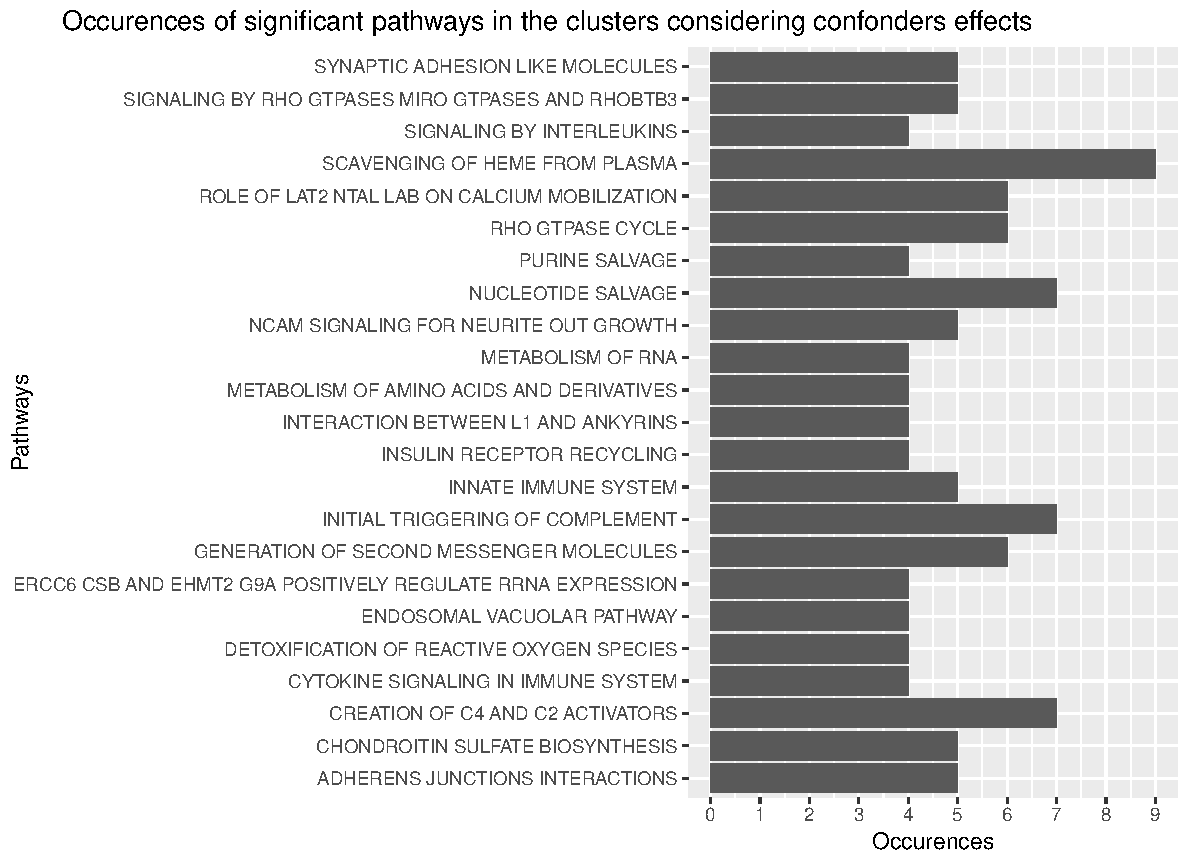
\includegraphics[width=\columnwidth]{figures/final_analysis/PathwaysWithConf}
	\caption{Pathways present in at least 4 clusters}
	\label{fig:path}
\end{figure}

Scavenging of heme from plasma is the pathway present in the greatest number of clusters. Free heme can have detrimental effects on tissues, causing cell damage by disrupting lipid bilayers through membrane intercalation, but also by promoting the conversion of low-density lipoproteins into cytotoxic oxidized products  \citep{reactomeReactomeScavenging}. These hemes are released into the plasma following intravascular hemolysis, a breakdown of erythrocytes in the blood vessels, releasing their constituents, including heme. Given that this pathway corresponds to a cellular protection system against a potential plasma constituent, a blood constituent, the clusters displaying this pathway (3, 9, 13, 16, 21, 22, 24 and 26) are probably made up of tiles from regions of the heart in direct contact with blood, i.e. the tissue lining the atria and ventricles. 

Nucleotide salvage corresponds to the reconversion of nucleosides and bases released by DNA and RNA degradation into nucleotide monophosphates, enabling them to be used again for nucleotide biosynthesis \citep{reactomeReactomeNucleotide}. Under normal conditions, this nucleotide salvage pathway should not function to any great extent, as DNA does not need to be intensively renewed. Nevertheless, the presence of this pathway in the top 10 in 7 clusters could indicate the presence of certain pathologies. For example, hyperactivity in nucleotide synthesis is a characteristic of cancer cells (ref), which could indicate that the donors from which the tiles making up these various clusters (0, 2, 3, 4, 16, 21, 29) originate could be carriers of some form of cancer. 

The initial triggering of complement is a pathway also present in 7 clusters. It is a signaling pathway involved in the recognition of infectious agents by the immune system and the induction of proteolysis, the degradation of foreign proteins \citep{Mullen2023}. This recognition can induce an inflammatory reaction that is potentially dangerous for the patient. The particularly high expression of this pathway in particular clusters (3, 9, 13, 15, 16, 22, 26) could indicate that a number of patients died as a result of a pathology directly impacting the heart, or which was severe enough to involve the heart in addition to other organs or regions of the body.

The creation of C4 and C2 activators is a pathway which, as its name suggests, activates the C4 and C2 immune complexes. These complementary components play an important role in the immune system. For example, an excess or a deficiency in C4 expression can have a major impact on a patient's immunity: a deficiency leads to impaired immune memory, while an excess exacerbates this immune response \citep{Blanchong2001}. The clusters showing overexpression of this pathway (3, 5, 9, 15, 16, 22 and 26) would therefore be made up of tiles from patients who had experienced a greater-than-normal immune response, which would have either caused death or been a pathological symptom.

\begin{table*}[t]
\footnotesize
\makebox[\linewidth]{
\begin{tabular}{|c |c |c |c| c | c| c|}
\cline{1-5}
    \hline & \multicolumn{1}{c|}{\rotatebox{90}{AGE adjusted for  COHORT }} &  \multicolumn{1}{c|}{\rotatebox{90}{SEX adjusted for DTHHRDY  } }  & \multicolumn{1}{c|}{\rotatebox{90}{HGHT adjusted for DTHHRDY }} & \multicolumn{1}{c|}{\rotatebox{90}{WGHT adjusted for DTHHRDY }} & \multicolumn{1}{c|}{\rotatebox{90}{BMI adjusted for DTHHRDY + COHORT }}  \\
    \hline 
\rotatebox{90}{Cluster} &
  \rotatebox{0}{Categorical (56+ vs -56)} &
  \rotatebox{0}{Female vs Male} &
  \rotatebox{0}{Categorical (71+ vs -71)} &
  \rotatebox{0}{Categorical (181+ vs -181)} &
  \rotatebox{0}{Categorical (28+ vs -28)}  \\
  \hline
0 &  &  & &  &   \\
1 &  &  &  &  &      \\
2 &  &  &  &   & \\
3 &  &  &  &  &    \\
4 &  &  &  &  &   \\
5 &  &  &  &  &   \\
6 &  &  &  & \cellcolor[HTML]{B4F5F2}-1,02 &\\
7 &  &  &  &  &    \\
8 &  &  & &  &   \\
9 &  &  &  &  &   \\
10 &  &  &  \cellcolor[HTML]{B4F5F2}-1.32 & \cellcolor[HTML]{B4F5F2}-1.41 \\
11 &  &  &  &  &   \\
12 &  &  &  &  &    \\
13 &  &  &  &  &   \\
14 &  &  &  &  &  \\
15 &  &  &  &  &   \\
16 &  &  &  &  &    \\
17 &  &  &  &  &   \\
18 &  &  &  &  &   \\
19 &  &  &  &  &    \\
20 &  &  &  &  &  \\
21 &  &  &  &  &   \\
22 &  &  &  &  &  \\
23 &  &  & &  &  \\
24 &  &  &  &  &  \\
25 &  &  & &  &\\
26 &  &  &  &  &   \\
27 &  &  &  &  \cellcolor[HTML]{FDFF89}1.07 &  \\
28 &  &  &  &  & \\
29 &  &  &  &  & \\
30 &  &  &  &  &  \\
31 &  &  &  &  &  \\
\hline
\end{tabular}}
\caption{Significant fold changes for each non-technical variable adjusted for their confounding technical variables.}
\label{tab:Q2bFC}
\end{table*}




\bibliography{references}

\end{multicols}
\end{document}